%\title{Presentation Template}
\documentclass[10pt]{beamer}

\usetheme[progressbar=frametitle]{metropolis}
\usepackage{appendixnumberbeamer}

\usepackage[compatibility=false]{caption}
\usepackage{subcaption}
\usepackage{csquotes}
\usepackage{booktabs}
\usepackage{hyperref}
\usepackage[scale=2]{ccicons}
\usepackage{tikz}
\usepackage{bm}

\usepackage{caption}
\captionsetup{justification=raggedright,singlelinecheck=false}

\usepackage{sidecap}
\sidecaptionvpos{figure}{c}

\usepackage{fontawesome}

\usepackage{footnpag} %reset footnotes at every page

\makeatother
\renewcommand{\thefootnote}{\ifcase\value{footnote}\or*\or
**\or***\or****\fi}
\makeatletter

\usepackage{xmpmulti}
\usepackage{pgffor}
\usepackage{multimedia}
\usepackage{media9}

\graphicspath{{./img/}}

\usepackage{pgfplots}
\usepgfplotslibrary{dateplot}

\usepackage{xspace}
\newcommand{\themename}{\textbf{\textsc{metropolis}}\xspace}

\definecolor{extralightgray}{gray}{0.85}

\title{Learning an Evolvable Genotype-Phenotype Mapping}
\subtitle{BEACON Congress 2018}
\date{August 10, 2018}
\author{Matthew Andres Moreno \newline {\faTwitter} @MorenoMatthewA \newline}
\titlegraphic{\vspace{32ex}\hfill\includegraphics[height=2.5cm]{img/BEACON-logo}}

\usepackage{fix-cm}

\makeatletter\newcommand\HUGE{\@setfontsize\Huge{28}{34}}\makeatother

\definecolor{h1}{HTML}{d19a66}
\definecolor{h2}{HTML}{36a8b8}

\usepackage{xcolor}

\begin{document}

\maketitle

% \begin{frame}{Table of contents}
%   \setbeamertemplate{section in toc}[sections numbered]
%   \tableofcontents[hideallsubsections]
% \end{frame}

\section{Autoencoders}

\begin{frame}{We Interrupt Your Regularly Scheduled Programming\dots}

\begin{columns}
\begin{column}{0.1\textwidth}
\end{column}
{%
\setlength{\fboxrule}{3pt}
\fcolorbox{lightgray}{extralightgray}{
\begin{column}{0.8\textwidth}
\centering
\begin{minipage}{0.9\textwidth}
\raggedright
\Large
\vspace{2ex}
The paper seems to be about autoencoders, not evolutionary algorithms.
\vskip5mm
\raggedleft
\large
--- Reviewer \#4\\
\vspace{2ex}
\end{minipage}

\end{column}
}
}
\begin{column}{0.1\textwidth}
\end{column}
\end{columns}

\end{frame}
\begin{frame}{We Interrupt Your Regularly Scheduled Programming\dots}

\begin{columns}
\begin{column}{0.1\textwidth}
\end{column}
{%
\setlength{\fboxrule}{3pt}
\fcolorbox{lightgray}{extralightgray}{
\begin{column}{0.8\textwidth}
\centering
\begin{minipage}{0.9\textwidth}
\raggedright
\Large
\vspace{2ex}
We'll use autoencoders to do cool evolution things, I promise!
\vskip5mm
\raggedleft
\large
--- me\\
\vspace{2ex}
\end{minipage}

\end{column}
}
}
\begin{column}{0.1\textwidth}
\end{column}
\end{columns}

\end{frame}

\begin{frame}{Autoencoder Intuition}

\vspace{1ex}
{\Large
\textbf{What does an autoencoder do?}%
\only<5>{%
\footnote{not just for faces!}
}
}%

\vspace{1ex}

\begin{figure}


\begin{columns}
\begin{column}{0.4\textwidth}
\onslide<2->{

\includegraphics[width=\textwidth]{guy}
}
\end{column}
\begin{column}{0.2\textwidth}
\onslide<3->{
\centering
\Large
auto encoder\\[1ex]

\includegraphics[width=\textwidth]{arrow}
}
\end{column}
\begin{column}{0.4\textwidth}
\onslide<4->{

\includegraphics[width=\textwidth]{curly-guy/latent-6}
}
\end{column}
\end{columns}
\vspace{1ex}

\begin{columns}
\begin{column}{0.4\textwidth}
\onslide<2->{
\Large
\centering
input
}
\end{column}
\begin{column}{0.2\textwidth}
\end{column}
\begin{column}{0.4\textwidth}
\onslide<4->{
\Large
\centering
reconstructed input
}
\end{column}
\end{columns}

\vspace{1ex}
\onslide<2->{
\caption{
Autoencoders take an input and then return a reconstructed input.
Graphics from \cite{white2016sampling}.
}
}
\end{figure}
\vspace{-3ex}
\end{frame}

\begin{frame}{Autoencoder Intuition}

{\Large
\textbf{Why are autoencoders useful?}
}

\pause

\vspace{4ex}

{\Large
two superpowers:

\pause

\begin{enumerate}

\item compression \onslide<5->{\textcolor{h2}{$\leftarrow$ bottlenecked autoencoder}}

\pause

\item de-corruption \onslide<6>{\textcolor{h2}{$\leftarrow$ denoising autoencoder}}

\end{enumerate}
}

\end{frame}

\begin{frame}{Autoencoder Intuition: Bottlenecked}

\begin{figure}

  \centering

  \begin{columns}
  \begin{column}{0.25\textwidth}
  \Large
  \centering
  \phantom{input}
  
\includegraphics[width=\textwidth]{img/guy}\\
  input
  \end{column}
  \begin{column}{0.5\textwidth}
  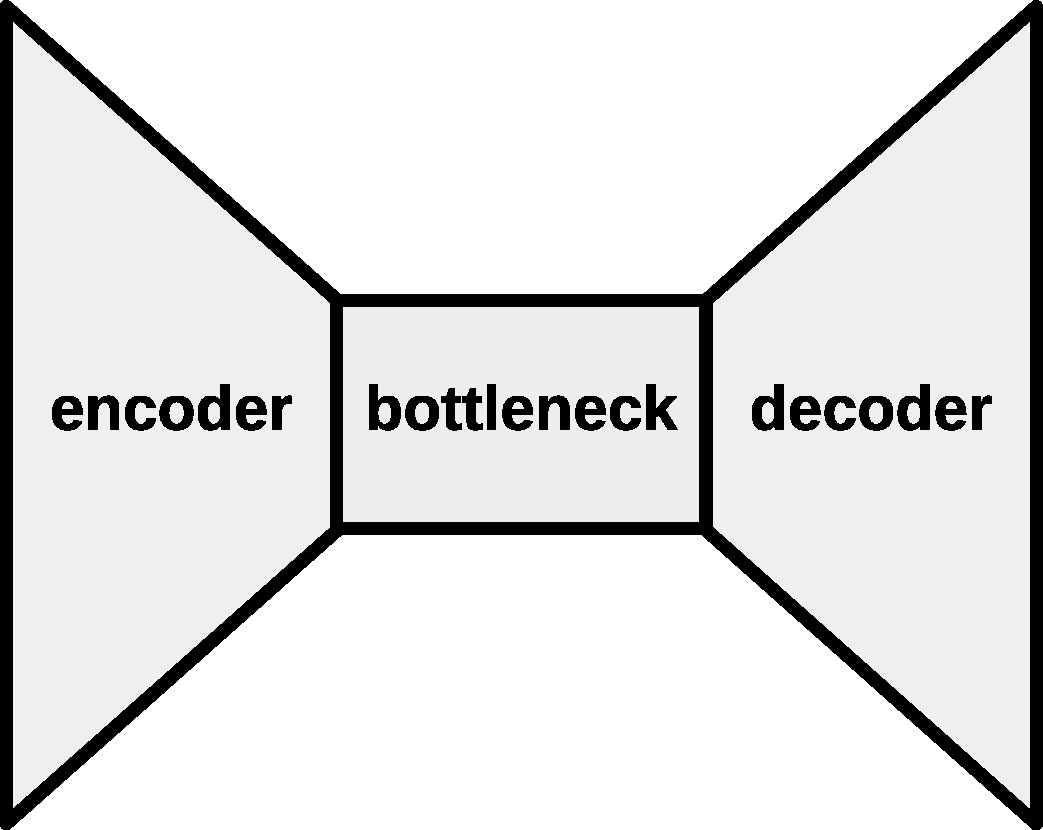
\includegraphics[width=\textwidth]{img/stripped_bottleneck}
  \end{column}
  \begin{column}{0.25\textwidth}
  \Large
  \centering
  ~\\[1.35ex]
  \phantom{input}
  
\includegraphics[width=\textwidth]{img/curly-guy/latent-6}\\
  reconst \\ input
  \end{column}
  \end{columns}

  \vspace*{-9.35ex}

  \makebox(0,0){
    
\includegraphics[width=0.1\textwidth]{static/static-1}\hspace{0.075ex}
  }

  \vspace*{9.35ex}


  \caption{
  Summary of bottlenecked autoencoders, which generate a compact encoding  (greyscale matrix) of a particular class of input (e.g., faces) then reconstruct the presented input.
  Graphics from \cite{white2016sampling}.
  }
\end{figure}

\end{frame}

\begin{frame}{Autoencoder Intuition: Bottlenecked}

\begin{figure}

  \begin{columns}
  \begin{column}{0.07\textwidth}
  \end{column}
  \begin{column}{0.6\textwidth}
  \small
  \centering
  \begin{columns}
  \begin{column}{0.225\textwidth}
  \centering
  input
  \end{column}
  \begin{column}{0.2\textwidth}
  \centering
  encoder
  \end{column}
  \begin{column}{0.15\textwidth}
  \centering
  bottle neck
  \end{column}
  \begin{column}{0.2\textwidth}
  \centering
  decoder
  \end{column}
  \begin{column}{0.225\textwidth}
  \centering
  reconst input
  \end{column}
  \end{columns}

  \vspace{1ex}

  \begin{columns}
  \begin{column}{0.225\textwidth}
  \centering
  
\includegraphics[width=\textwidth]{guy}
  \end{column}
  \begin{column}{0.2\textwidth}
  \centering
  
\includegraphics[width=0.75\textwidth]{arrow}
  \end{column}
  \begin{column}{0.15\textwidth}
  \centering
  
\includegraphics[width=\textwidth]{static/static-1}
  \end{column}
  \begin{column}{0.2\textwidth}
  \centering
  
\includegraphics[width=0.75\textwidth]{arrow}
  \end{column}
  \begin{column}{0.225\textwidth}
  \centering
  
\includegraphics[width=\textwidth]{curly-guy/latent-6}
  \end{column}
  \end{columns}

  \vspace*{1.5ex}

  \makebox(0,0){
    $\bm{\vdots}$
  }

  \vspace*{3.25ex}

  \begin{columns}
  \begin{column}{0.225\textwidth}
  \end{column}
  \begin{column}{0.2\textwidth}
  \end{column}
  \begin{column}{0.15\textwidth}
  \centering
  
\includegraphics[width=\textwidth]{static/static-2}
  \end{column}
  \begin{column}{0.2\textwidth}
  \centering
  
\includegraphics[width=0.75\textwidth]{arrow}
  \end{column}
  \begin{column}{0.225\textwidth}
  \centering
  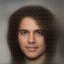
\includegraphics[width=\textwidth]{curly-guy/latent-3}
  \end{column}
  \end{columns}

  \vspace*{1.5ex}

  \makebox(0,0){
    $\bm{\vdots}$
  }

  \vspace*{3.25ex}

  \begin{columns}
  \begin{column}{0.225\textwidth}
  \centering
  
\includegraphics[width=\textwidth]{curly}
  \end{column}
  \begin{column}{0.2\textwidth}
  \centering
  
\includegraphics[width=0.75\textwidth]{arrow}
  \end{column}
  \begin{column}{0.15\textwidth}
  
\includegraphics[width=\textwidth]{static/static-3}
  \end{column}
  \begin{column}{0.2\textwidth}
  \centering
  
\includegraphics[width=0.75\textwidth]{arrow}
  \end{column}
  \begin{column}{0.225\textwidth}
  \centering
  
\includegraphics[width=\textwidth]{curly-guy/latent-1}
  \end{column}
  \end{columns}

  \end{column}
  \begin{column}{0.03\textwidth}
  \end{column}
  \begin{column}{0.3\textwidth}
  \caption{
  ~\\
  Summary of latent space interpolation.
  Intermediate bottlenecked encodings between two input images are visualized.
  Graphics from \cite{white2016sampling}.
  }
  \end{column}
  \end{columns}

\end{figure}

\end{frame}

\begin{frame}{Autoencoder Intuition: Bottlenecked}

\begin{figure}

\begin{columns}
\begin{column}{0.6\textwidth}
\foreach \n in {1,...,12}{%
\includegraphics<\n>[width=\textwidth]{latent-walk/latent-\n}%
}%
\end{column}
\begin{column}{0.4\textwidth}
\caption{
Frame-by-frame latent space interpolation animation.
Graphics from \cite{white2016sampling}.
}
\end{column}
\end{columns}

\end{figure}

\end{frame}


\begin{frame}{Autoencoder Intuition: Denoising}

\begin{figure}

\begin{columns}
\begin{column}{0.3\textwidth}
\includegraphics<1>[width=\textwidth]{reconstruct/original-senior}
\includegraphics<2->[width=\textwidth]{reconstruct/corrupted-senior}
\end{column}
\begin{column}{0.4\textwidth}
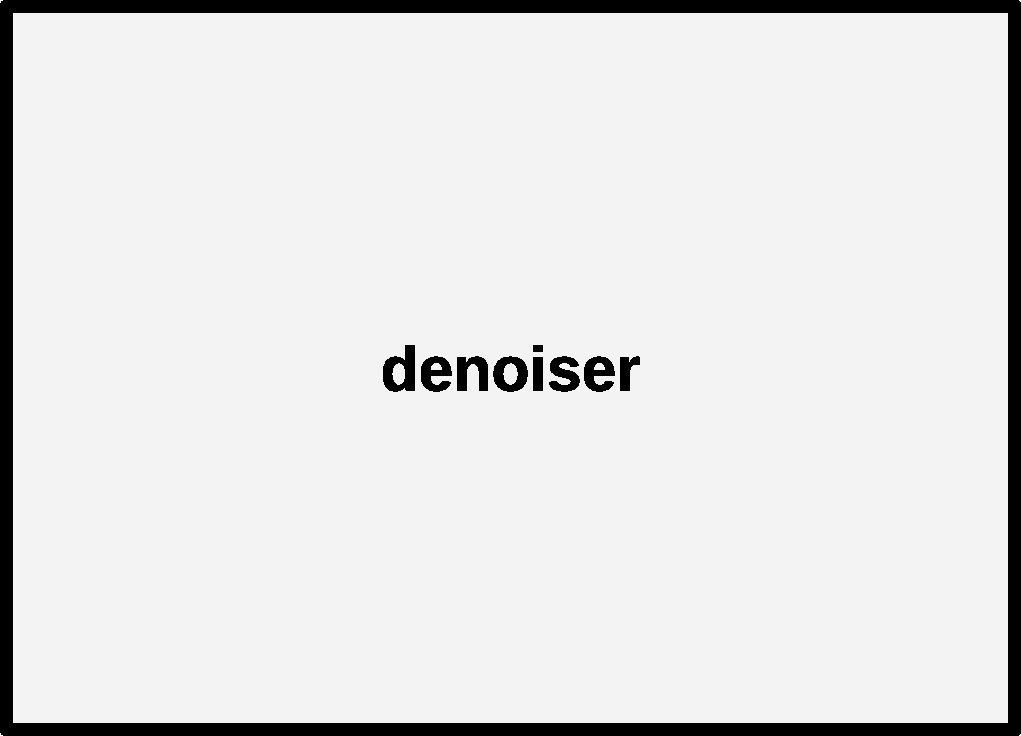
\includegraphics[width=\textwidth]{stripped_denoiser}
\end{column}
\begin{column}{0.3\textwidth}
\includegraphics[width=\textwidth]<3->{reconstruct/reconstructed-senior}
\end{column}
\end{columns}

\vspace{1ex}

\begin{columns}
\begin{column}{0.3\textwidth}
\centering
\only<1>{input}
\only<2->{corrupted input}
\end{column}
\begin{column}{0.4\textwidth}
\end{column}
\begin{column}{0.3\textwidth}
\centering
\only<1,2>{\phantom{reconst input}}
\only<3->{reconst input}
\end{column}
\end{columns}

\vspace{1ex}

\caption{
Summary of denoising autoencoder, which receives a corrupted copy of a particular class of input (e.g., faces) and attempts to recover the uncorrupted input.
Graphics from \cite{allen2018generative}.
}
\end{figure}

\end{frame}


\begin{frame}{Autoencoder Implementation}

\Large

\textbf{What's under the hood?}

\pause

\vspace{3ex}
\centering

\HUGE
\onslide<3->{%
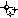
\includegraphics[width=1em]{emoji-star}%
}%
~deep learning
\onslide<3->{%
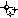
\includegraphics[width=1em]{emoji-star}%
}

\normalsize
\onslide<4->{
(a.k.a. big artificial neural networks + big training data)
}

\end{frame}

\begin{frame}{Autoencoder Implementation: Training}
\begin{figure}
\includegraphics[width=0.8\textwidth]{celeba}
\caption{
Training requires a large, representative set of examples of the class of objects to autoencode.
Graphic from \cite{liu2015faceattributes}.
}
\end{figure}
\end{frame}

\section{Automap: Using Autoencoders to Learn an Evolvable Genotype-Phenotype Map}

\begin{frame}{Remember This?}

\begin{figure}
\begin{subfigure}[b]{\textwidth}
\foreach \n in {6,...,1}{%
\includegraphics[width=0.167\textwidth]{straight-guy/latent-\n}%
}%
\caption{latent-space interpolation}
\end{subfigure}

\uncover<2>{
\begin{subfigure}[b]{\textwidth}
\foreach \n in {1,...,6}{%
\includegraphics[width=0.167\textwidth]{straight-guy/linear-\n}%
}%
\caption{pixel-space interpolation}
\end{subfigure}
}

\caption{
Comparison of latent- and pixel-space interpolations.
Graphics adapted from \cite{white2016sampling}.
}
\end{figure}

\end{frame}

\begin{frame}{Bottlenecked G-P Map: Implementation}

\begin{figure}
  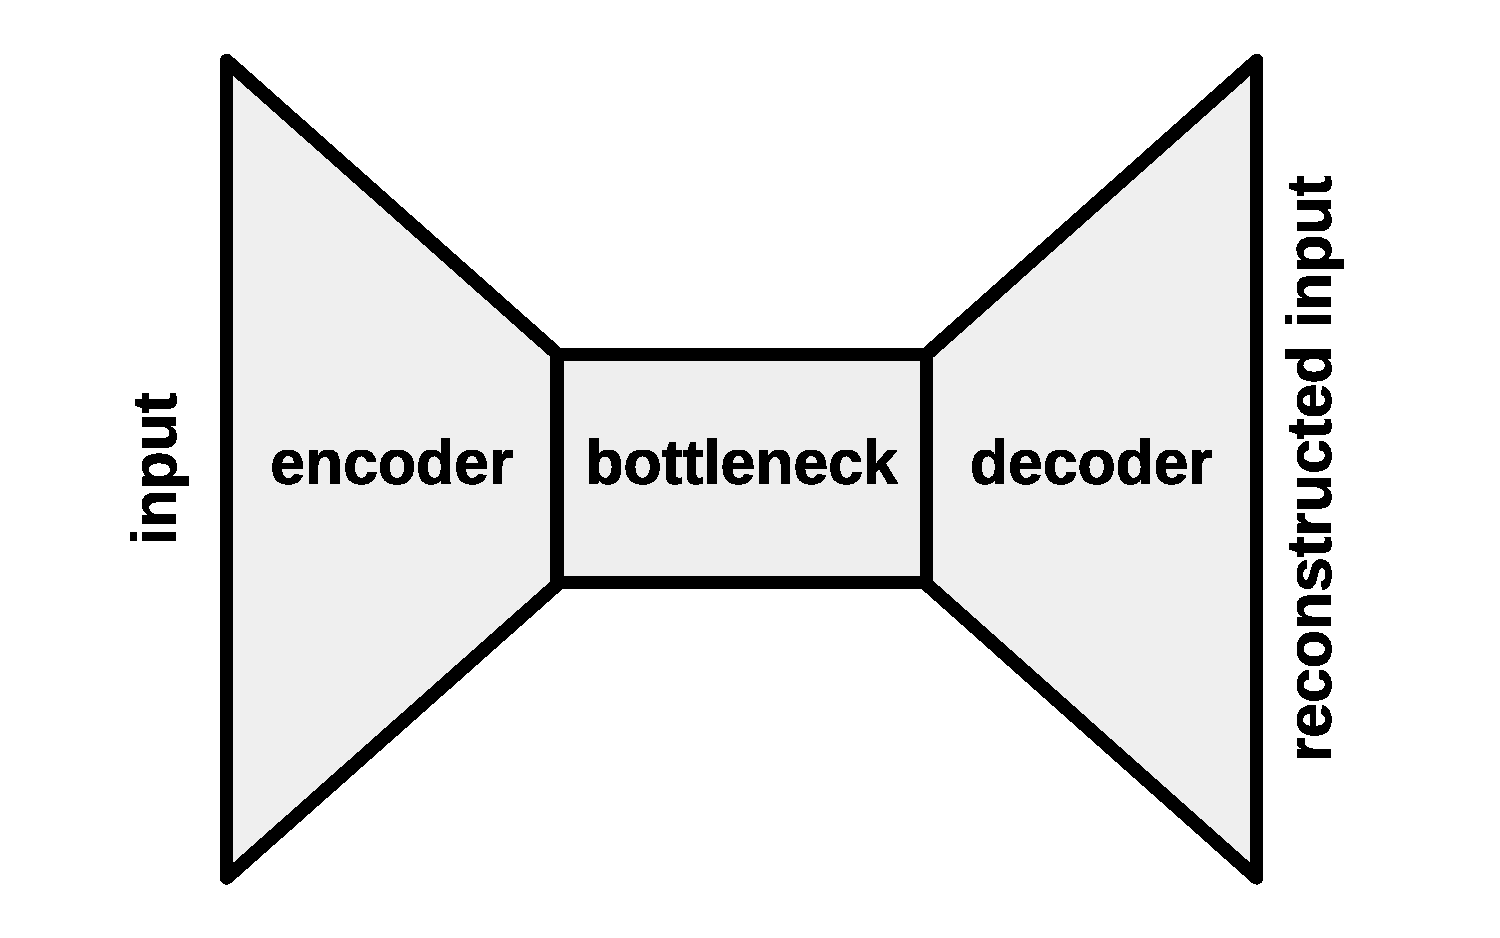
\includegraphics[width=\linewidth]{img/bottleneck}
  \caption{
    Schematic of a bottlenecked autoencoder.
  }\label{fig:bottleneck}
\end{figure}


\end{frame}

\begin{frame}{Bottlenecked G-P Map: Implementation}

\begin{figure}
  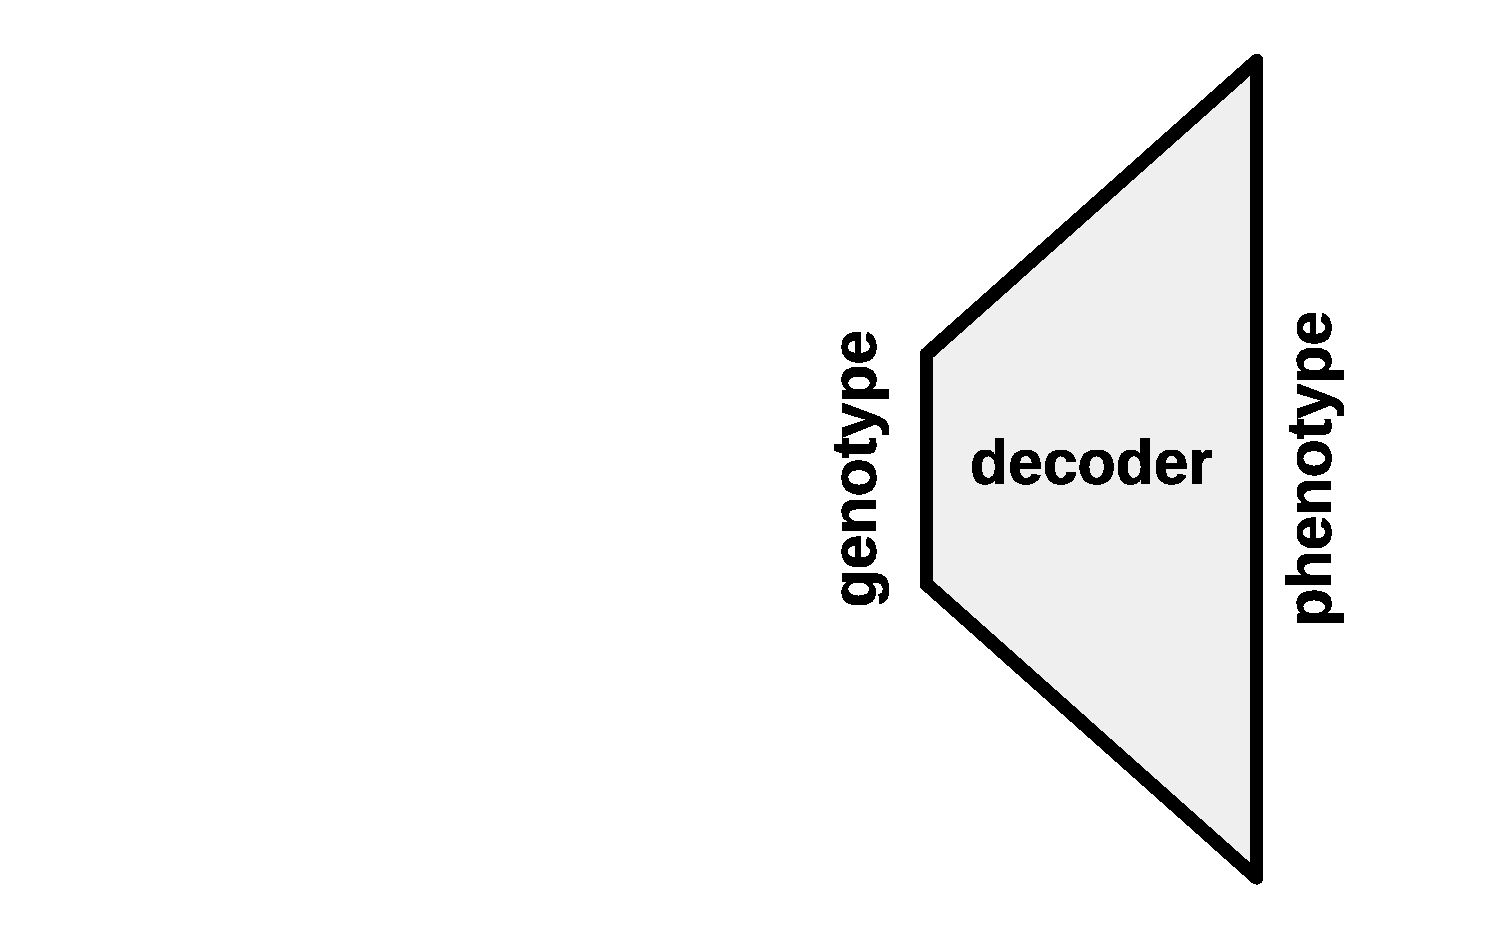
\includegraphics[width=\linewidth]{img/bottleneck_map}
  \caption{
    Schematic of a genotype-phenotype map constructed with a bottlenecked autoencoder.
  }\label{fig:bottleneck_map}
\end{figure}


\end{frame}

\begin{frame}{Bottlenecked G-P Map: Evolvability}
\begin{figure}
\begin{columns}
\begin{column}{0.7\textwidth}
  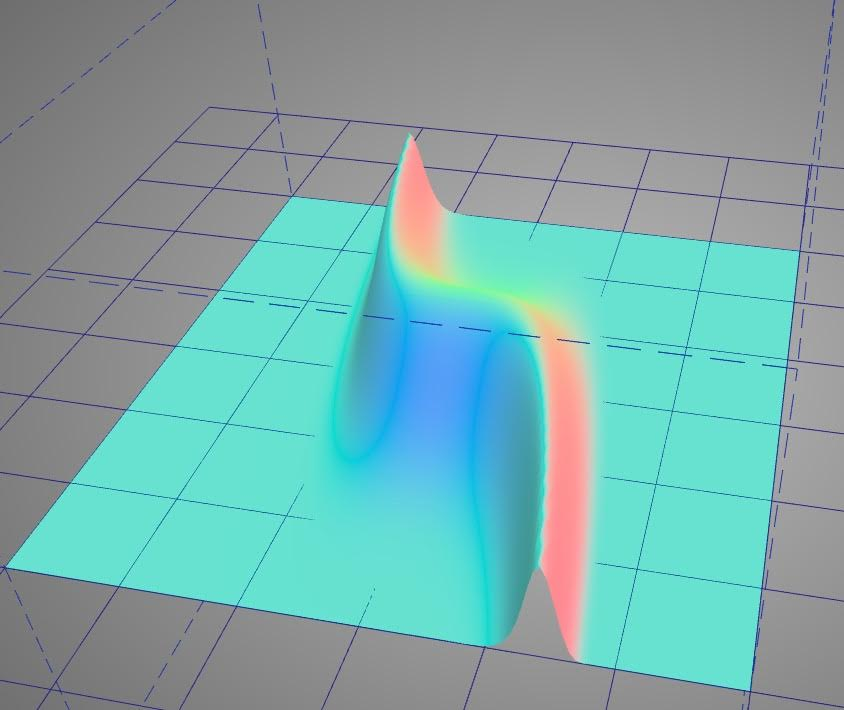
\includegraphics[width=\textwidth]{landscape-bottleneck/landscape-1}%
\end{column}
\begin{column}{0.3\textwidth}
\caption{
A hypothetical fitness landscape.
}
\end{column}
\end{columns}
\end{figure}
\end{frame}

\begin{frame}{Bottlenecked G-P Map: Evolvability}
\begin{figure}
\begin{columns}
\begin{column}{0.7\textwidth}
  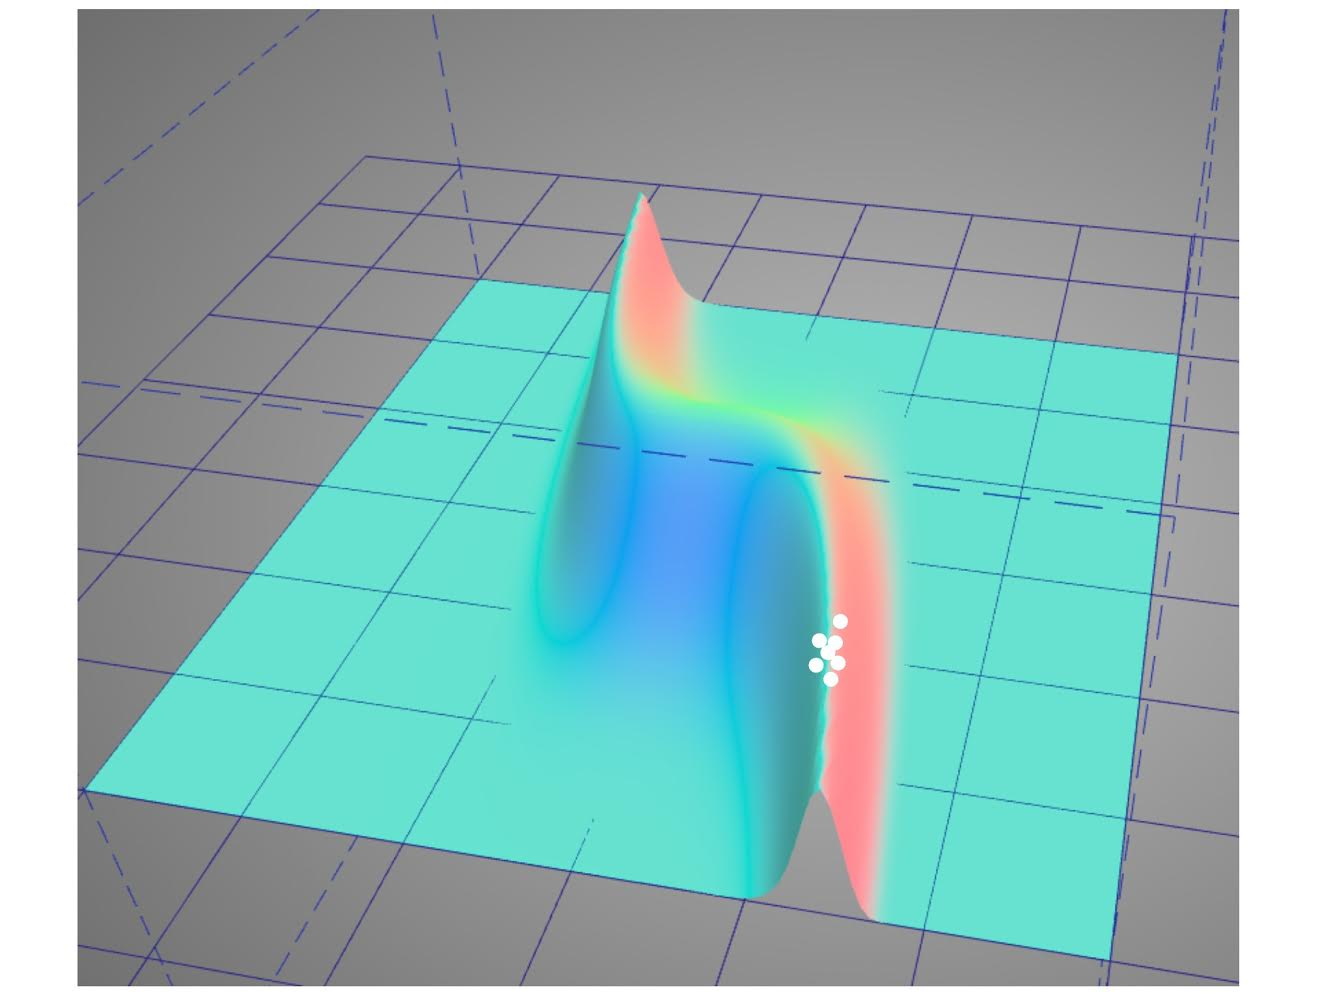
\includegraphics[width=\textwidth]{landscape-bottleneck/landscape-2}%
\end{column}
\begin{column}{0.3\textwidth}
\caption{
Hypothetical evolutionary end-state of a single population on a fitness landscape.
}
\end{column}
\end{columns}
\end{figure}
\end{frame}

\begin{frame}{Bottlenecked G-P Map: Evolvability}
\begin{figure}
\begin{columns}
\begin{column}{0.7\textwidth}
  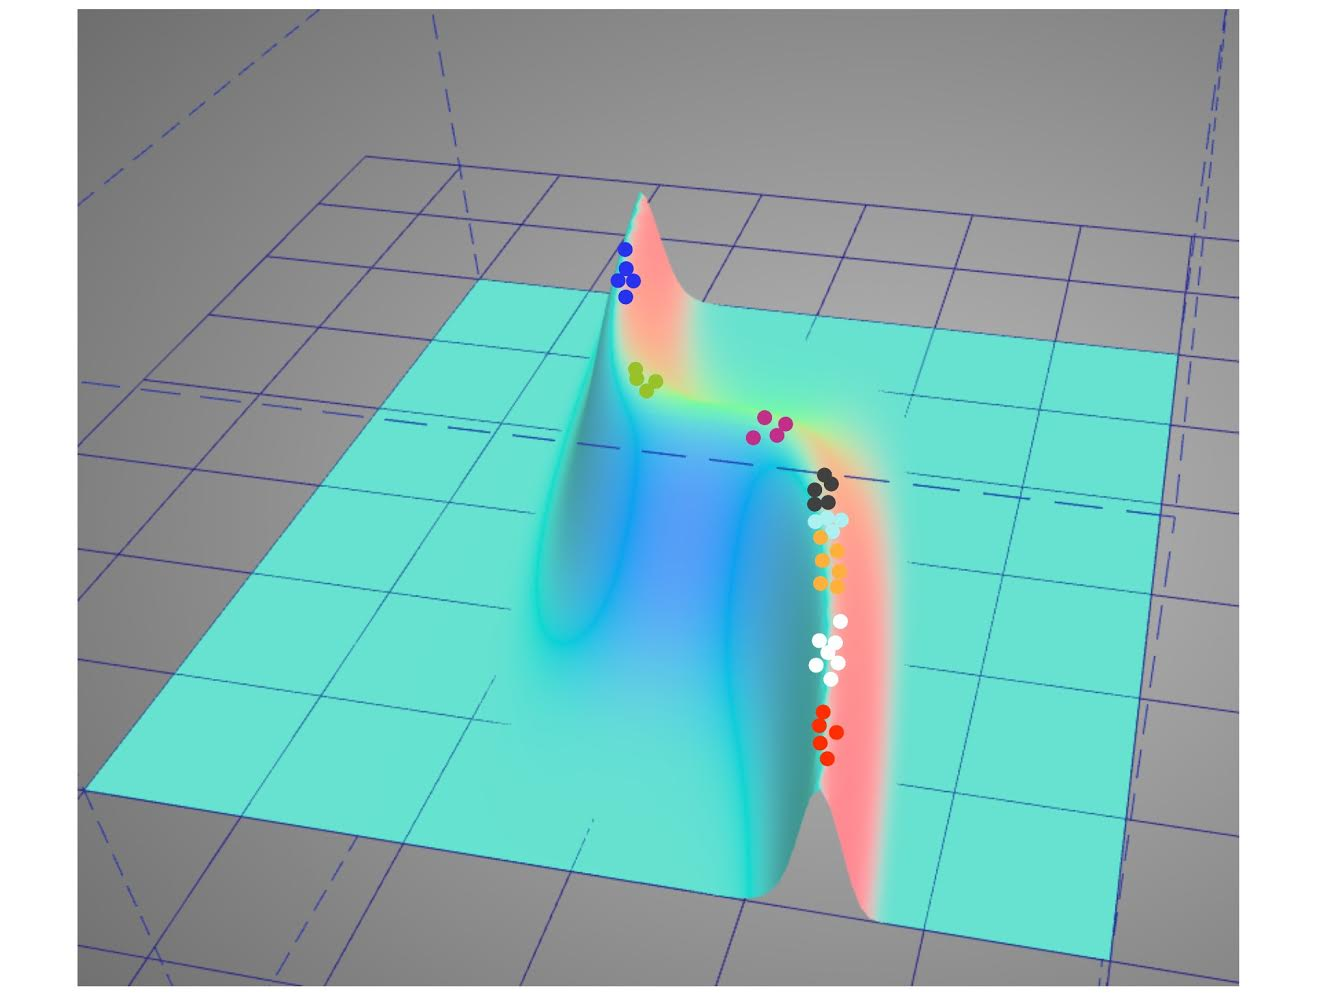
\includegraphics[width=\textwidth]{landscape-bottleneck/landscape-3}%
\end{column}
\begin{column}{0.3\textwidth}
\caption{
Hypothetical evolutionary end-state of several populations on a fitness landscape.
}
\end{column}
\end{columns}
\end{figure}
\end{frame}

\begin{frame}{Bottlenecked G-P Map: Evolvability}
\begin{figure}
  \includegraphics<1>[width=\textwidth,trim={0 4cm 0 4cm },clip]{landscape-bottleneck/landscape-4}%
  \includegraphics<2>[width=\textwidth,trim={0 4cm 0 4cm },clip]{landscape-bottleneck/landscape-5}%
  \includegraphics<3>[width=\textwidth,trim={0 4cm 0 4cm },clip]{landscape-bottleneck/landscape-6}%
  \includegraphics<4>[width=\textwidth,trim={0 4cm 0 4cm },clip]{landscape-bottleneck/landscape-7}%
  \includegraphics<5>[width=\textwidth,trim={0 4cm 0 4cm },clip]{landscape-bottleneck/landscape-8}%
\caption{
Hypothetical mutational trajectory on a fitness landscape with denoising genotype-phenotype map.
}
\end{figure}
\end{frame}

\begin{frame}{Remember This?}
  \vspace{2ex}
  \begin{figure}
  \begin{columns}
  \begin{column}{0.3\textwidth}
  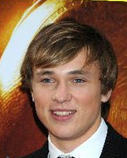
\includegraphics[width=\textwidth]{reconstruct/original-boy}
  \end{column}
  \begin{column}{0.05\textwidth}
  \centering
  \rotatebox{90}{Corrupt}\\
  
\includegraphics[width=\textwidth]{arrow}
  \end{column}
  \begin{column}{0.3\textwidth}
  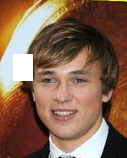
\includegraphics[width=\textwidth]{reconstruct/corrupted-boy}
  \end{column}
  \begin{column}{0.05\textwidth}
  \centering
  \rotatebox{90}{Autoencoder}\\
  
\includegraphics[width=\textwidth]{arrow}
  \end{column}
  \begin{column}{0.3\textwidth}
  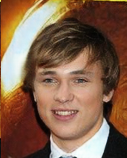
\includegraphics[width=\textwidth]{reconstruct/reconstructed-boy}
  \end{column}
  \end{columns}
  \vspace{1ex}
  \caption{
  Autoencoder restoring masked section of image.
  Graphics from \cite{white2016sampling}.
  }
  \end{figure}

\end{frame}

\begin{frame}{Denoising G-P Map: Implementation}

\begin{figure}
  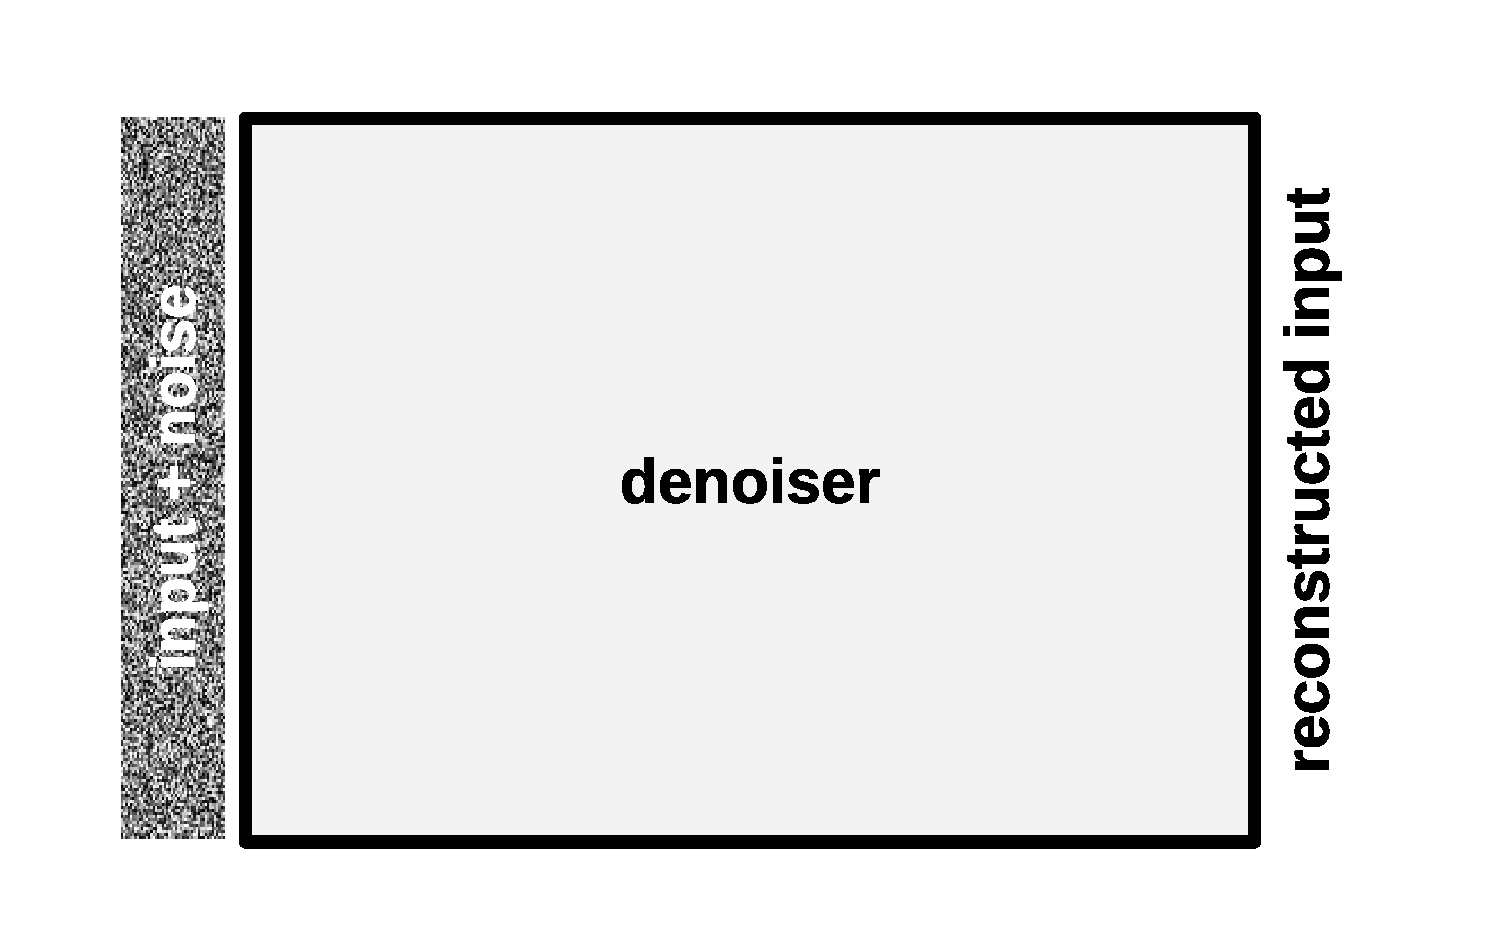
\includegraphics[width=\linewidth]{img/denoiser}
  \caption{
    Schematic of a denoising autoencoder.
  }\label{fig:denoiser}
\end{figure}


\end{frame}

\begin{frame}{Denoising G-P Map: Implementation}

\begin{figure}
  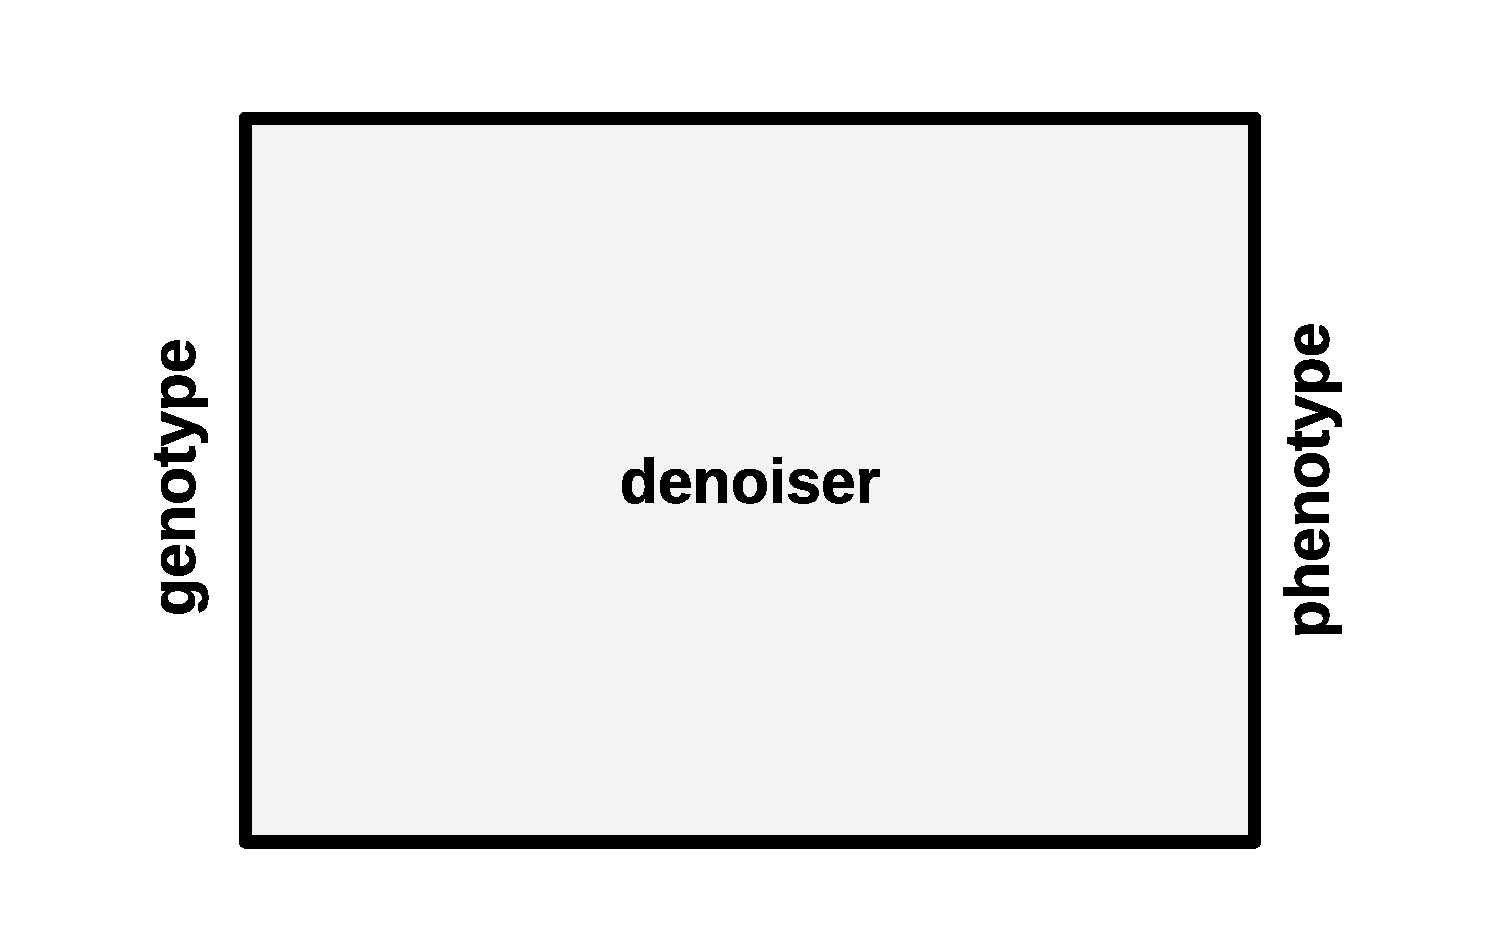
\includegraphics[width=\linewidth]{img/denoiser_map}
  \caption{
    Schematic of a genotype-phenotype map constructed with a denoising autoencoder.
  }\label{fig:denoiser_map}
\end{figure}


\end{frame}

\begin{frame}{Denoising G-P Map: Evolvability}

\begin{figure}

\begin{columns}
\begin{column}{0.6\textwidth}
  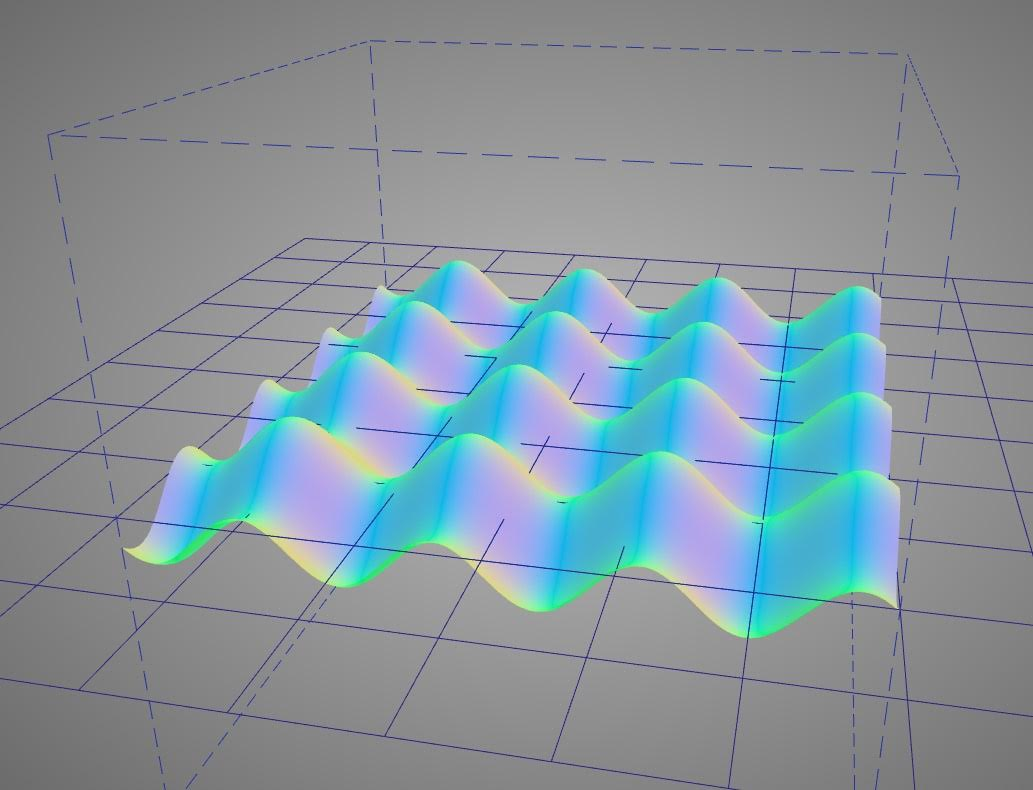
\includegraphics[width=\textwidth]{landscape-denoise/landscape-1}%
\end{column}
\begin{column}{0.4\textwidth}
\caption{
A hypothetical fitness landscape.
}
\end{column}
\end{columns}

\end{figure}

\end{frame}
\begin{frame}{Denoising G-P Map: Evolvability}

\begin{figure}

\begin{columns}
\begin{column}{0.6\textwidth}
  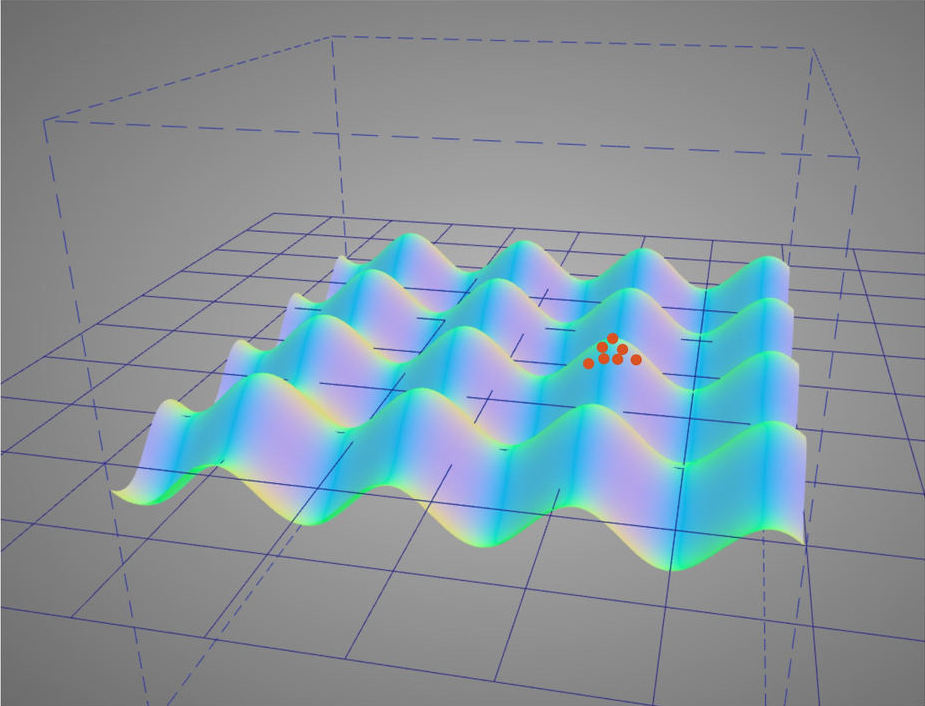
\includegraphics[width=\textwidth]{landscape-denoise/landscape-2}%
\end{column}
\begin{column}{0.4\textwidth}
\caption{
Hypothetical evolutionary end-state of a single population on a fitness landscape.
}
\end{column}
\end{columns}

\end{figure}

\end{frame}
\begin{frame}{Denoising G-P Map: Evolvability}

\begin{figure}

\begin{columns}
\begin{column}{0.6\textwidth}
  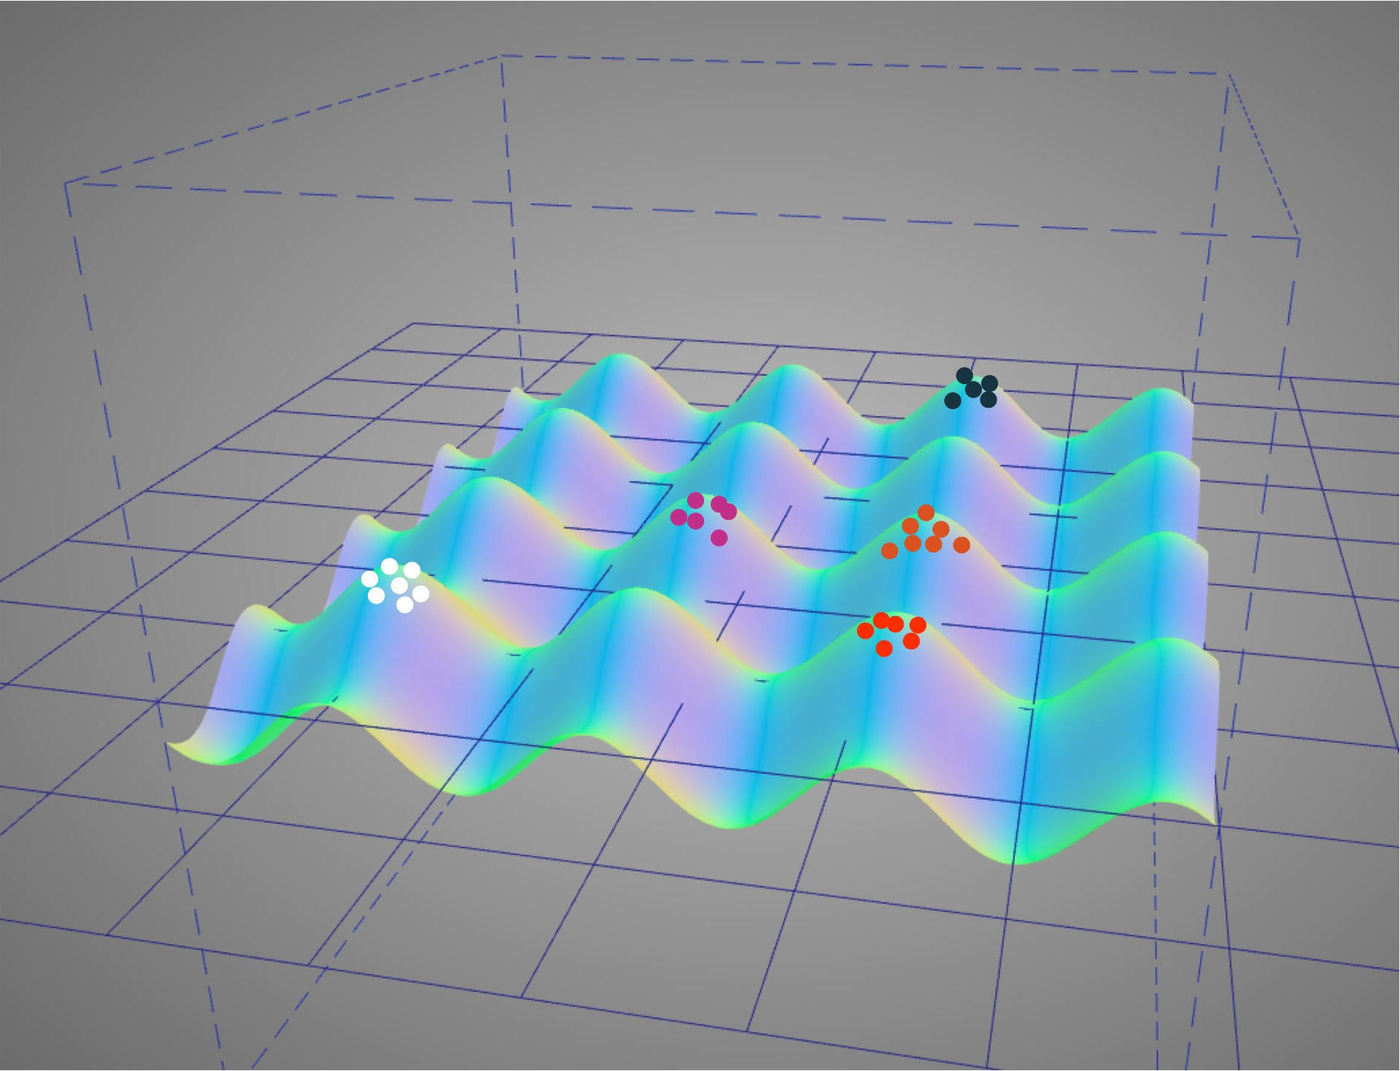
\includegraphics[width=\textwidth]{landscape-denoise/landscape-3}%
\end{column}
\begin{column}{0.4\textwidth}
\caption{
Hypothetical evolutionary end-state of several populations on a fitness landscape.
}
\end{column}
\end{columns}

\end{figure}

\end{frame}
\begin{frame}{Denoising G-P Map: Evolvability}

\begin{figure}
  \begin{columns}
  \begin{column}{0.6\textwidth}
  \includegraphics<1>[width=\textwidth]{landscape-denoise/landscape-4}%
  \includegraphics<2>[width=\textwidth]{landscape-denoise/landscape-5}%
  \includegraphics<3>[width=\textwidth]{landscape-denoise/landscape-6}%
  \includegraphics<4>[width=\textwidth]{landscape-denoise/landscape-7}%
  \includegraphics<5>[width=\textwidth]{landscape-denoise/landscape-8}%
\end{column}
\begin{column}{0.4\textwidth}
\caption{
Hypothetical mutational trajectory on a fitness landscape with denoising genotype-phenotype map.
}
\end{column}
\end{columns}

\end{figure}

\end{frame}

\begin{frame}{Autoencoder G-P Maps: Training}
\Large

We need examples of good solutions to train autoencoder.

\pause

How to get training data?

\pause

\begin{itemize}[<+->]
\item survey local fitness peaks
\begin{itemize}
  \item repeated evolutionary runs with direct encoding
  \item repeated evolutionary runs with manually-designed indirect encoding
\end{itemize}
\item harness pre-existing data
\begin{itemize}
  \item ex. face images
\end{itemize}
\end{itemize}

\end{frame}

\section{Final Thoughts}

\begin{frame}{Automap: Challenges (\& Solutions?)}

\textbf{If you already need good solutions to train, why use automap?}
\pause
\vspace{-1ex}
\begin{itemize}[<+->]
\itemsep0em
\item might yield even better solutions (``needle in the haystack'')
\item perhaps try iterative bootstrapping of G-P autoencoder maps in absence of good solutions
\end{itemize}
\vspace{-1ex}
\pause
\textbf{Can automap only generate the good solutions used to train?}
\pause
\vspace{-1ex}
\begin{itemize}[<+->]
\itemsep0em
\item deep learning can often generalize beyond training data
\item mix and match elements of good solutions
\end{itemize}

\end{frame}

\appendix

\begin{frame}{For More Information}

\vspace{1ex}

{\HUGE\url{https://osf.io/n92c7/}}

\vspace{3ex}

\begin{itemize}
\item source code
\item data
\item figures and graphics
\item how-to-replicate tutorial
\item publication
\item slides
\item blog article
\end{itemize}

\end{frame}

\begin{frame}{People}

\vspace{1ex}

\begin{columns}
\begin{column}{0.25\textwidth}
  \centering
  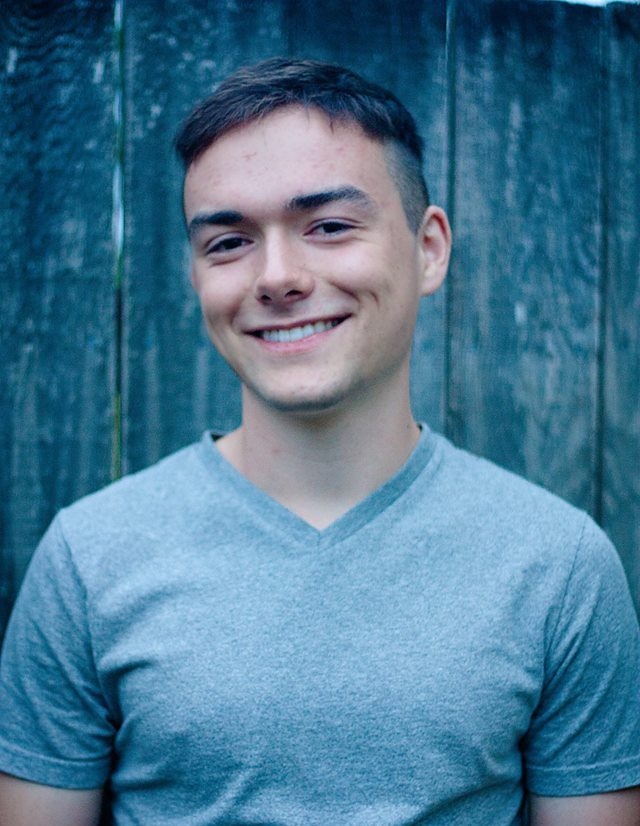
\includegraphics[width=0.7\textwidth,trim={0 15 0 15},clip]{moreno}
\end{column}
\begin{column}{0.75\textwidth}
  \textbf{Matthew Andres Moreno}

  \href{https://twitter.com/MorenoMatthewA}{{\faTwitter} @MorenoMatthewA}

  \href{https://mmore500.github.io}{{\faGlobe} \texttt{https://mmore500.github.io}}

  \href{mailto: mmore500@msu.edu}{{\faEnvelope} \texttt{mmore500@msu.edu}}

\end{column}
\end{columns}

\vspace{1ex}

\begin{columns}
\begin{column}{0.25\textwidth}
  \centering
  \includegraphics[width=0.7\textwidth,trim={0 100 0 50},clip]{banzhaf}
\end{column}

\begin{column}{0.75\textwidth}
  \textbf{Wolfgang Banzhaf}

  \href{http://www.cse.msu.edu/~banzhafw/}{{\faGlobe} \texttt{http://www.cse.msu.edu/\textasciitilde{}banzhafw/}}

  \href{mailto: banzhafw@msu.edu}{{\faEnvelope} \texttt{banzhafw@msu.edu}}

\end{column}
\end{columns}

\vspace{1ex}

\begin{columns}
\begin{column}{0.25\textwidth}
  \centering
  \includegraphics[width=0.7\textwidth]{ofria}
\end{column}

\begin{column}{0.75\textwidth}
  \textbf{Charles Ofria}

  \href{https://twitter.com/CharlesOfria}{{\faTwitter} @CharlesOfria}

  \href{https://ofria.com}{{\faGlobe} \texttt{https://ofria.com}}

  \href{mailto: ofria@msu.edu}{{\faEnvelope} \texttt{ofria@msu.edu}}

\end{column}
\end{columns}

\end{frame}

\begin{frame}{Acknowledgements}
\begin{itemize}
\item Distributed Evolutionary Algorithms for Python
package \cite{fortin2012deap}
\item PyTorch Deep Learning framework \cite{paszke2017pytorch}
\item Open Science Framework via the Center for Open Science
\item computational resources via Michigan State University's Institute for Cyber-Enabled Research
\item computational resources via Google Cloud Compute
\end{itemize}

\vfill

\newcommand{\innerspacer}{0.07\textwidth}
\newcommand{\content}{0.24\textwidth}
\newcommand{\outerspacer}{0.07\textwidth}

\begin{center}
 \begin{columns}
	\begin{column}{\outerspacer}~\end{column}
	 \begin{column}{\content}
		
\includegraphics[width=\textwidth]{NSF-logo}
 	\end{column}
  \begin{column}{\innerspacer}~\end{column}
	 \begin{column}{\content}
		\includegraphics[width=\textwidth]{BEACON-logo}
 	\end{column}
  \begin{column}{\innerspacer}~\end{column}
 	\begin{column}{\content}
   \includegraphics[width=0.75\textwidth]{MSU-helmet}
 	\end{column}
 	\begin{column}{\outerspacer}~\end{column}
 \end{columns}
\end{center}

\end{frame}


\begin{frame}[standout]

  \vspace{17ex}

  {\Huge
  Questions?
  }
  \vspace{15ex}

  \url{https://osf.io/n92c7/}

\end{frame}

\begin{frame}[allowframebreaks]{References}

  \bibliography{bibl}
  \setbeamertemplate{bibliography item}{\insertbiblabel}
  % \nocite{*} % Insert publications even if they are not cited in the poster
  \bibliographystyle{apalike}
\end{frame}

% \section{Evolvability \& Genotype-Phenotype Map}

\begin{frame}{Defining Evolvability}
consensus: the amount of \textcolor{h2}{viable} \textcolor{h1}{variation} generated by the evolutionary process
\begin{itemize}
  \item evolvability as the amount of \textcolor{h1}{\textbf{novel variation}} generated
  \item evolvability the proportion of variation that is \textcolor{h2}{\textbf{viable}}
\end{itemize}
\end{frame}

\begin{frame}{Evolvability: Novelty}


\begin{figure}
 \centering
    \begin{subfigure}[b]{0.5\textwidth}
        \centering
    	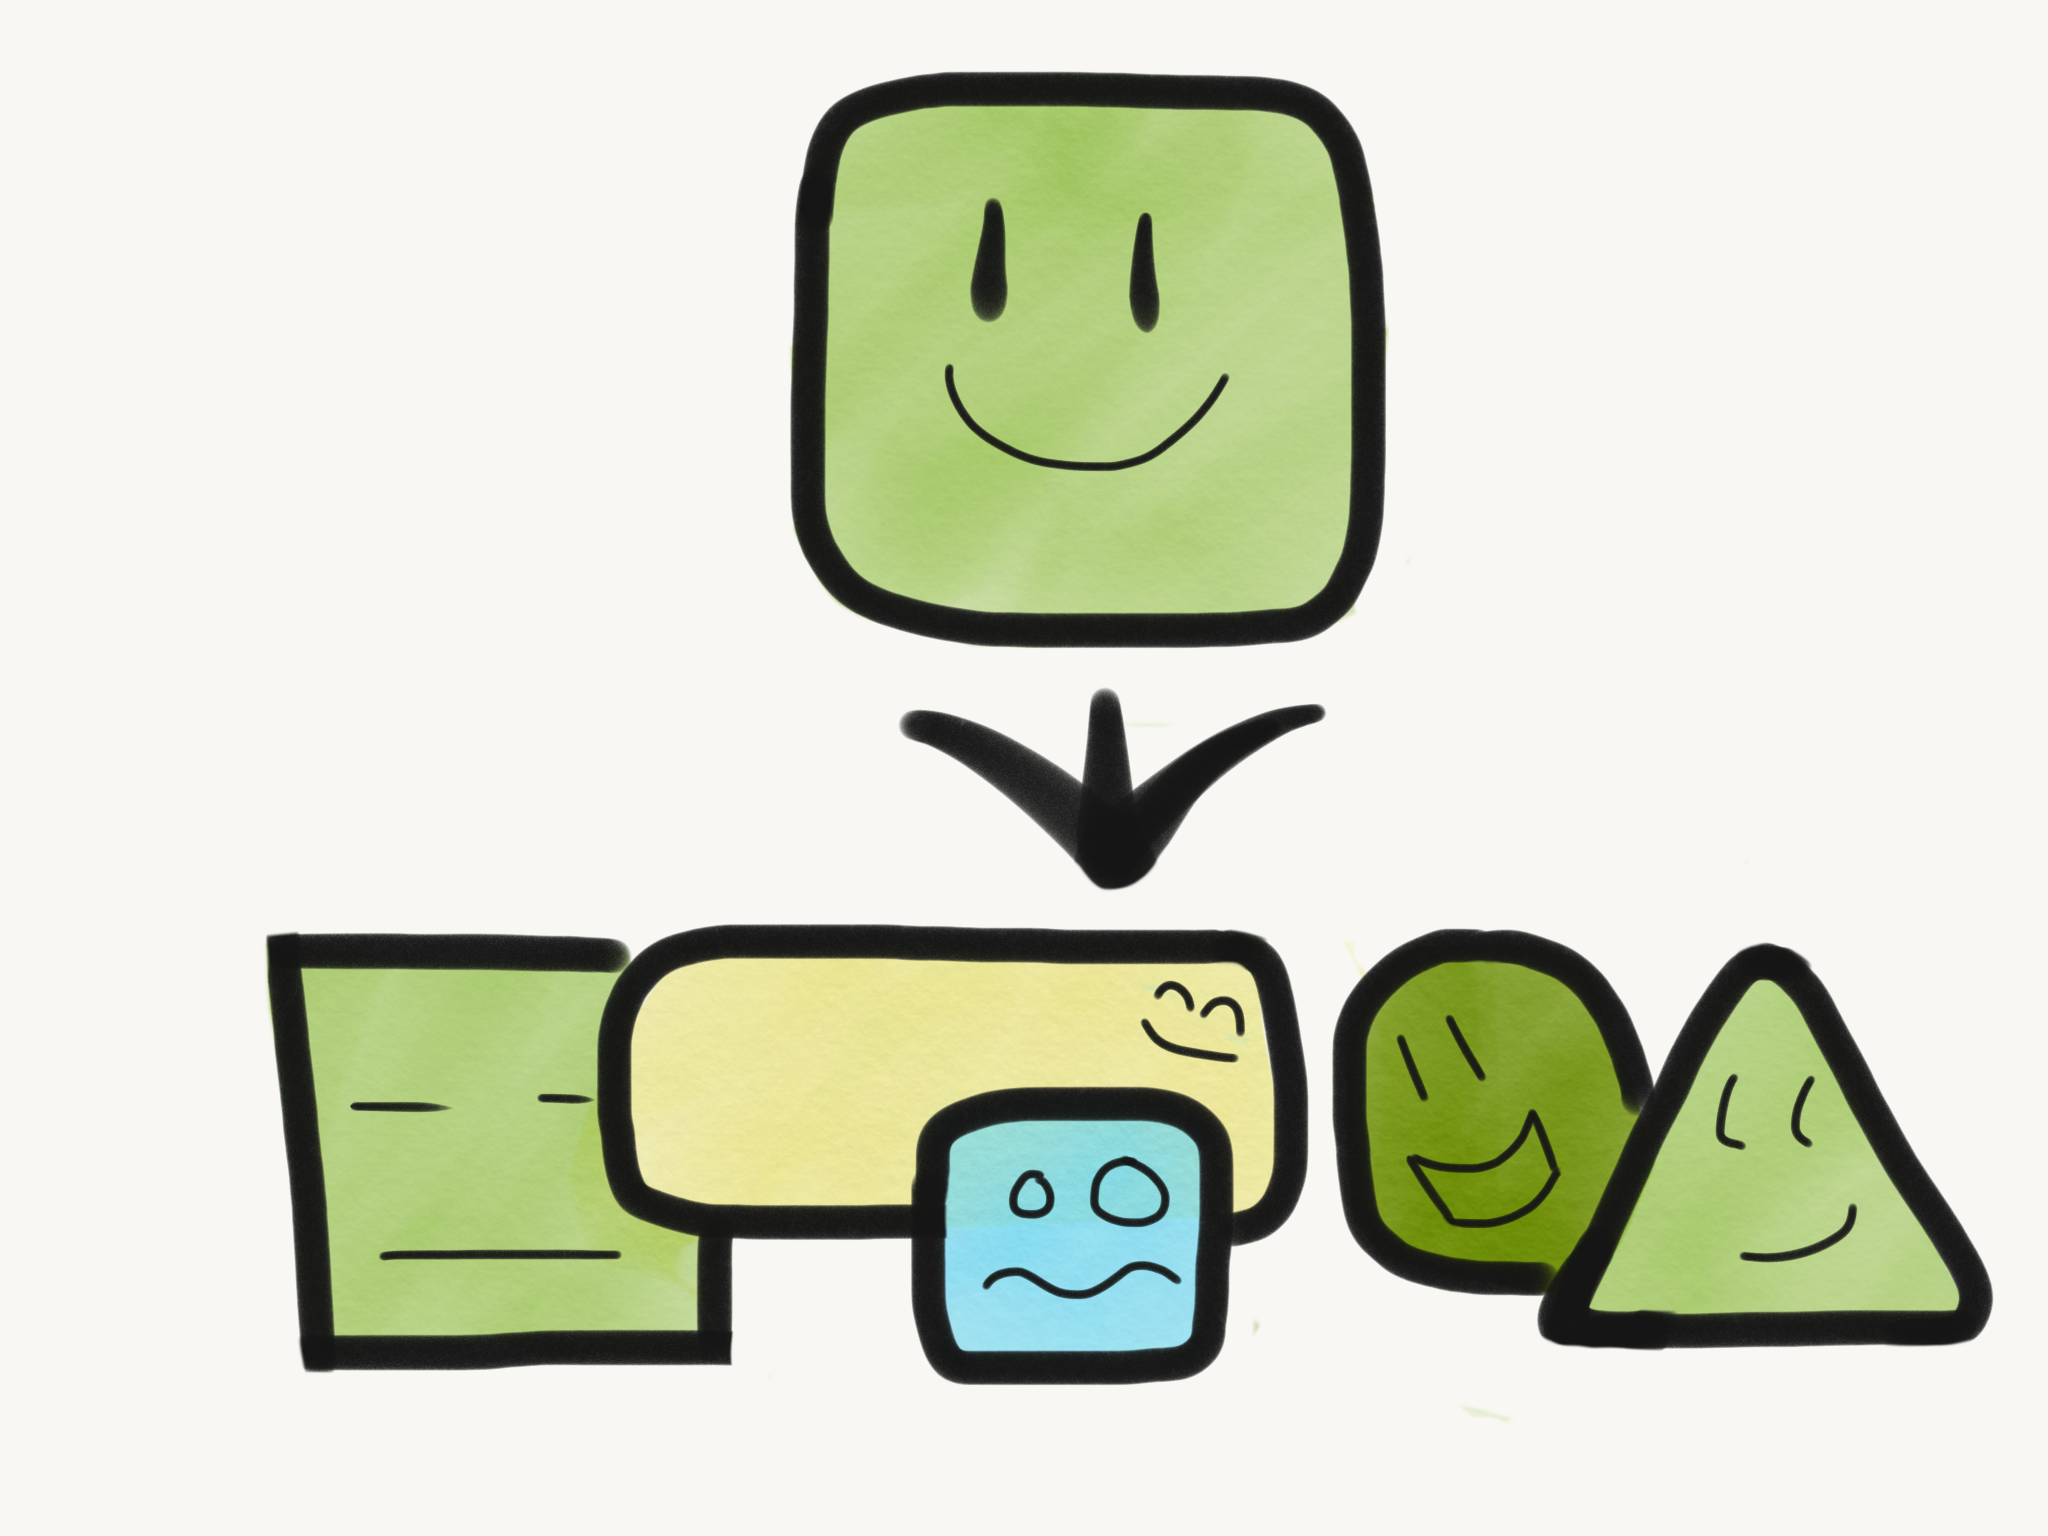
\includegraphics[width=\textwidth]{img/individual_evolvability}
        \caption{high phenotypic variation among offspring}
        \label{fig:high}
    \end{subfigure}%
    \hfill
    \begin{subfigure}[b]{0.5\textwidth}
        \centering
        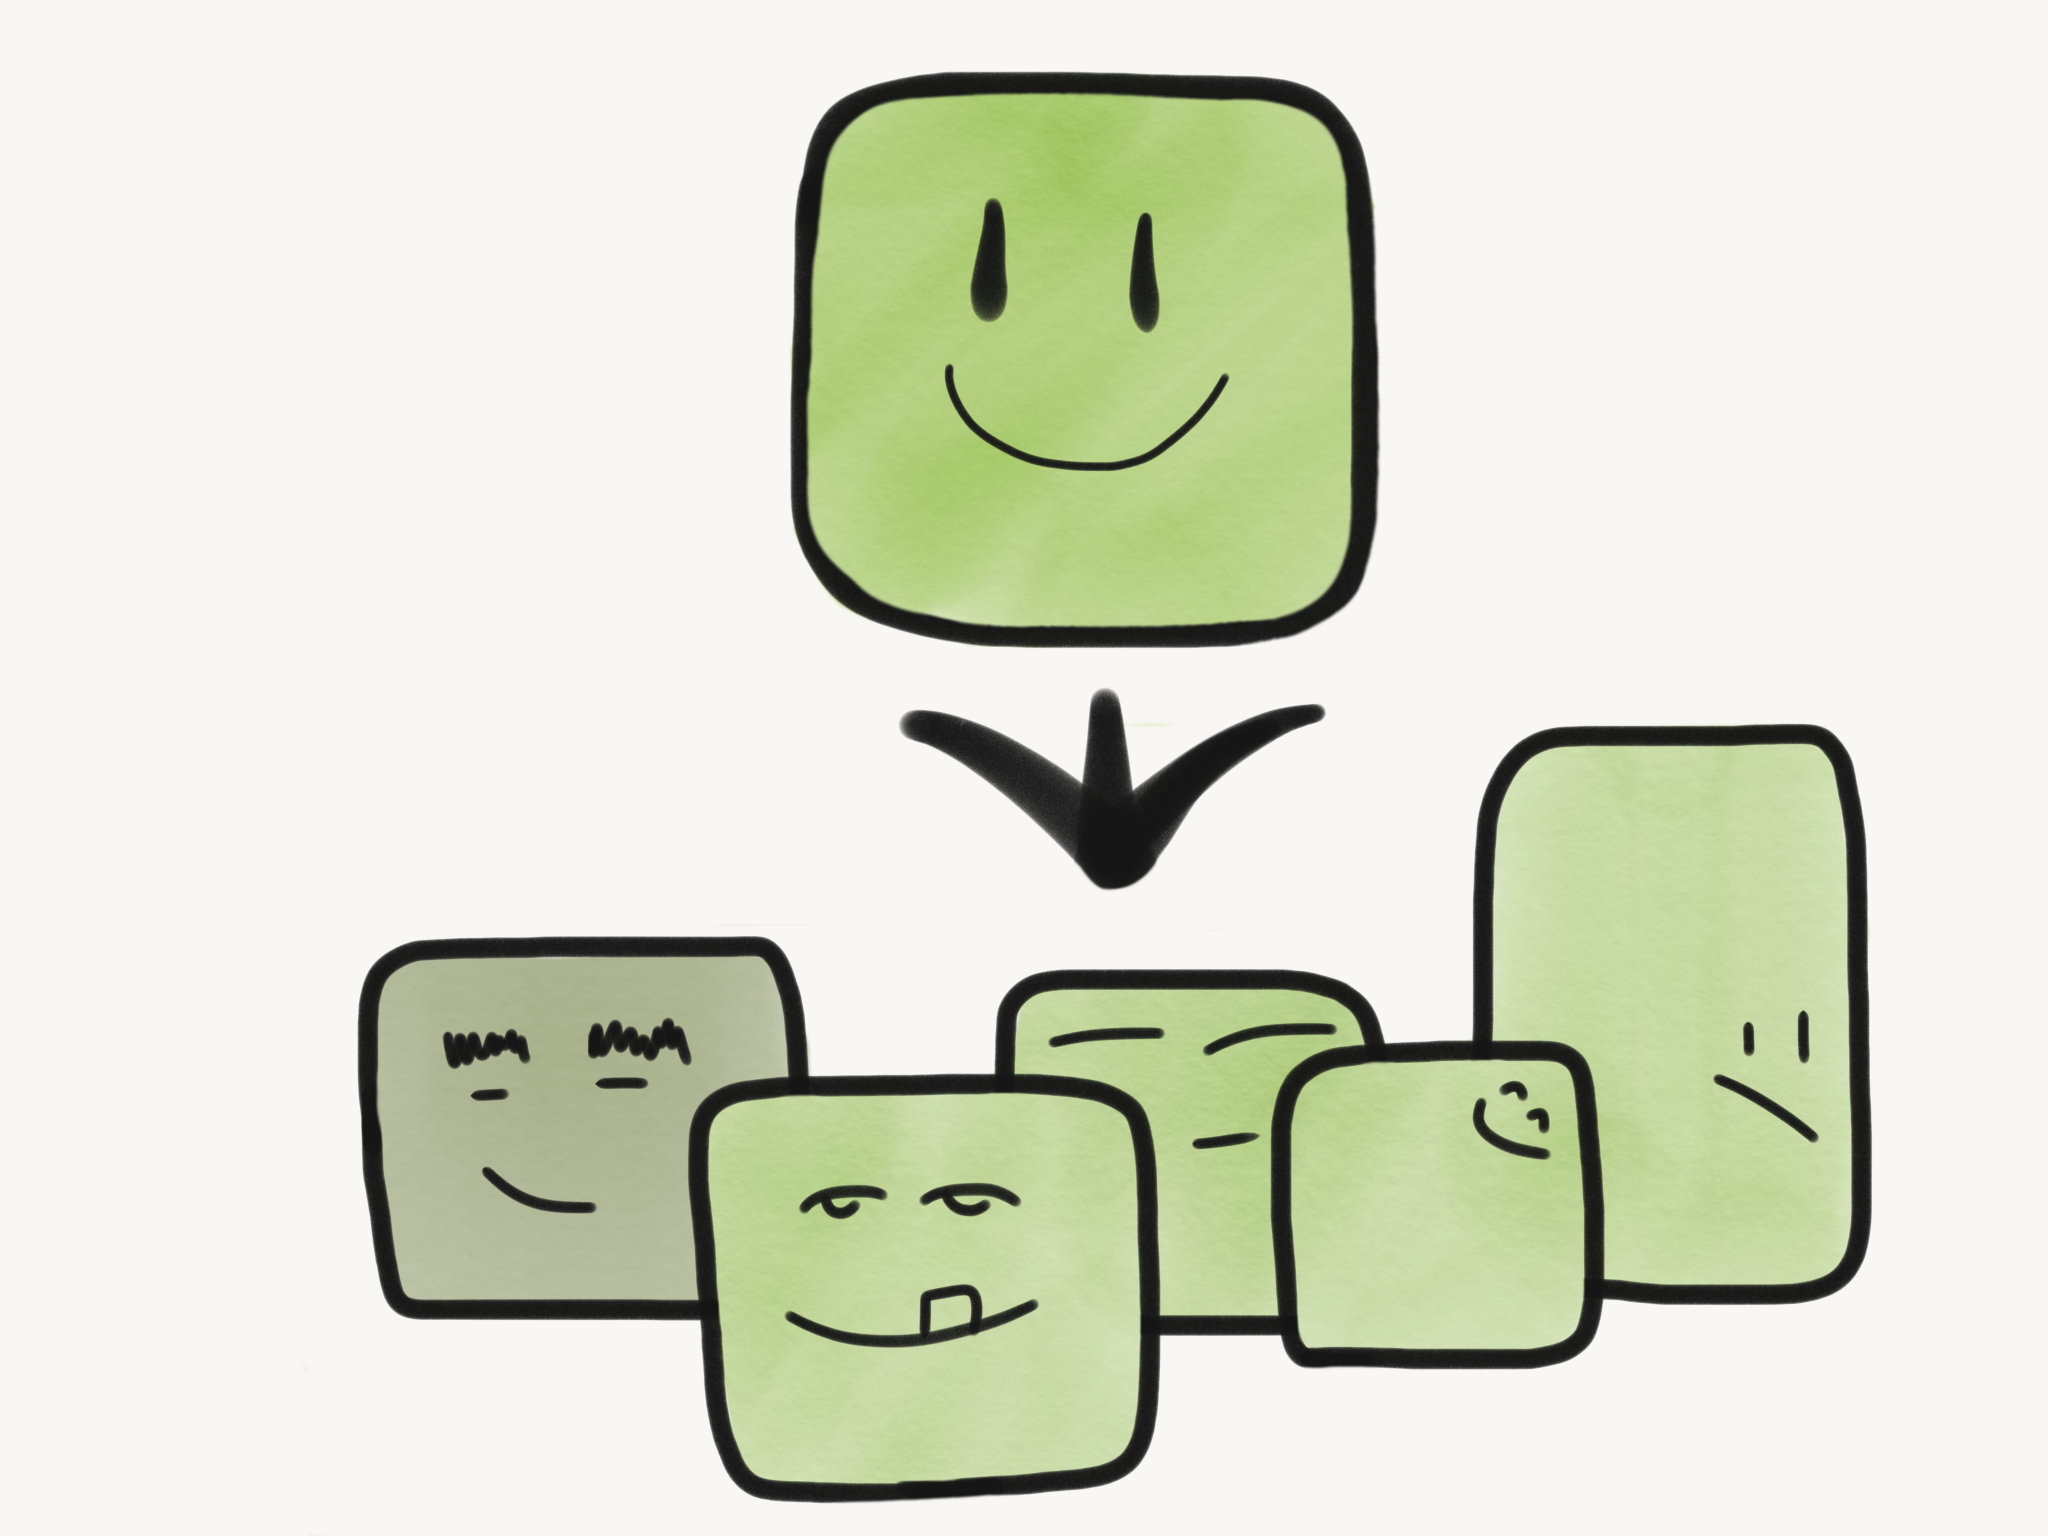
\includegraphics[width=\textwidth]{img/low_individual_evolvability}
        \caption{low phenotypic variation among offspring}
        \label{fig:low}
    \end{subfigure}
    \vspace{-4ex}
  \caption{An comparison of high (\ref{fig:high}) and low (\ref{fig:low}) levels of phenotypic variation under mutation; high evolvability left and low evolvability right.}
\end{figure}


\end{frame}

\begin{frame}{Evolvability: Viability}

\begin{figure}
    \centering
    \includegraphics[width=0.8\textwidth]{img/robustness}
 	\captionsetup{singlelinecheck=off,justification=raggedright}
  	\caption{Illustration of robustness under mutation; high evolvability left and low evolvability right.}
    \label{fig:robustness}
\end{figure}


\end{frame}

\begin{frame}{Evolvability \& Genotype-Phenotype Map}

\begin{figure}

\foreach \n in {1,...,4}{%
\includegraphics<\n>[width=0.8\textwidth]{gpmaps/even-\n}%
}%

\caption{
Graph of phenotypes connected by single-step mutations induced by a genotype-phenotype map.
Graphic inspired by \cite{ahnert2017structural}.
}

\end{figure}

\end{frame}

\begin{frame}{Evolvability \& Genotype-Phenotype Map}

\begin{figure}

\foreach \n in {1,...,4}{%
\includegraphics<\n>[width=0.8\textwidth]{gpmaps/filtered-\n}%
}%

\caption{
Graph of phenotypes connected by single-step mutations induced by a genotype-phenotype map.
Note the bias towards viability induced by exclusion of invalid phenotypes.
Graphic inspired by \cite{ahnert2017structural}.
}

\end{figure}

\end{frame}

\begin{frame}{Evolvability \& Genotype-Phenotype Map}

\begin{figure}

\foreach \n in {1,...,4}{%
\includegraphics<\n>[width=0.8\textwidth]{gpmaps/layered-\n}%
}%

\caption{
Graph of phenotypes connected by single-step mutations induced by a genotype-phenotype map.
Note the difficulty of traversing the region of invalid phenotypes.
Graphic inspired by \cite{ahnert2017structural}.
}

\end{figure}

\end{frame}

% \begin{frame}{Evolvability \& Genotype-Phenotype Map}
%
% \begin{figure}
%
% \foreach \n in {1,...,4}{%
% \includegraphics<\n>[width=0.8\textwidth]{gpmaps/rare-\n}%
% }%
%
% \caption{TODO Graphic inspired by \cite{ahnert2017structural}.}
%
% \end{figure}
%
% \end{frame}

\begin{frame}{Evolvability \& Genotype-Phenotype Map}

\begin{figure}

\foreach \n in {1,...,4}{%
\includegraphics<\n>[width=0.8\textwidth]{gpmaps/reduced-\n}%
}%

\caption{
Graph of phenotypes connected by single-step mutations induced by a genotype-phenotype map.
Note the dimensionality reduction.
Graphic inspired by \cite{ahnert2017structural}.
}

\end{figure}

\end{frame}

\begin{frame}{Evolvable Genotype-Phenotype Maps}

\Large

\textcolor{h2}{
In EC, we define the genotype-phenotype map.
}
\normalsize

\vspace{1ex}

\pause

\textbf{Option A:} use direct genotype-phenotype map
\pause
\begin{itemize}
\item often poor evolvability
\end{itemize}

\pause

\textbf{Option B:} use manually-designed indirect genotype-phenotype map
\pause
\begin{itemize}
\item labor-intensive
\item ad-hoc/heuristic
\item might be computationally prohibitive to evaluate
\item might still have poor evolvability$\dots$
\end{itemize}

\pause

\textbf{Option C?}

\end{frame}

\begin{frame}{Challenges + Solutions}

\textbf{Computational cost of making training data.}
\pause
\vspace{-1ex}
\begin{itemize}[<+->]
\itemsep0em
\item parallelism
\end{itemize}
\vspace{-1ex}
\pause


\textbf{Autoencoder performance limitations}
\pause
\vspace{-1ex}
\begin{itemize}[<+->]
\itemsep0em
\item ANN autoencoders: active area of research
\item G-P autoencoder map could use other ``back end''
\end{itemize}

\end{frame}

\begin{frame}{Toy Result: Evolvability Signature}

\begin{figure}
  \begin{subfigure}[b]{0.33\linewidth}
    \includegraphics[width=\linewidth]{img/results/direct_es_unscaled}
    \subcaption{
      direct map
    }\label{fig:table_direct_es}
  \end{subfigure}
  \begin{subfigure}[b]{0.33\linewidth}
    \includegraphics[width=\linewidth]{img/results/noise_es_unscaled}
    \subcaption{
      denoising map
    }\label{fig:table_noise_es}
  \end{subfigure}
  \begin{subfigure}[b]{0.33\linewidth}
    \includegraphics[width=\linewidth]{img/results/bottleneck_es_unscaled}
    \subcaption{
      bottleneck map
    }\label{fig:table_bottleneck_es}
  \end{subfigure}
  \caption{
    Evolvability signatures for three genotype-phenotype maps in the $n$-legged table problem domain.
    Note that subfigure \ref{fig:table_bottleneck_es} is presented with different axis scaling than subfigures \ref{fig:table_direct_es} and \ref{fig:table_noise_es}.
  }\label{fig:all_es}
\end{figure}


\end{frame}

\begin{frame}{TODO}

\begin{figure}
\foreach \n in {6,...,1}{%
\includegraphics[width=0.167\textwidth]{curly-guy/linear-\n}%
}%
\caption{TODO}
\end{figure}

\end{frame}

\begin{frame}{Result: Evolutionary Pacing}

\begin{figure}
  \includegraphics[width=0.8\linewidth]{img/results/scrabble_fit_vs_gen}
  \caption{
    Maximum individual fitness by generation in populations evolving in the Scrabble string domain.
    Bootstrapped 95\% confidence intervals are shaded along each curve.
  }\label{fig:scrabble_fit_vs_gen}
\end{figure}


\end{frame}


% \begin{frame}{Evolutionary Algorithm Parameters: Toy Problem}
%
% \begin{itemize}
% \item population size: 300
% \item tournament selection: $k = 5$
% \item crossover: two-point, two-parent, $p = 0.5$
% \item mutation: site-wise Gaussian perturbation
% \begin{itemize}
% \item training data, evolvability-signature experiments: $\mu = 0$, $\sigma = 0.1$, per-individual
% probability = 0.2, per-site probability = 0.01
% \item response-to-selection experiments: $\mu = 0$, $\sigma = 0.1$, per-individual probability = 0.2, per-site probability = 0.2 %TODO check this
% \footnote{for the bottleneck map, a per-site probability of 1 was employed}
% \end{itemize}
% \end{itemize}
%
% \end{frame}
%
% \begin{frame}{Denoising Autoencoder Hyperparameters: Toy Problem}
%
% \begin{itemize}
% \item 100-to-100 fully-connected linear layer without bias
% \item trained for 2500 epochs by stochastic gradient descent
% \item learning rate: $10^{−4}$
% \item momentum: 0.9
% \item batch size: 2048
% \item model parameters initialized uniformly between 0.005 and 0.015
% \item model parameters clamped in the range (0, 1
% \item during the training process, Gaussian
%   noise with $\mu = 0$, $\sigma = 0.025$ applied to input
% \item loss: mean square error of the difference between the original phenotype the reconstructed phenotype
% \end{itemize}
%
% \end{frame}
%
% \begin{frame}{Evolutionary Algorithm Parameters: Scrabble Problem}
%
% TODO
%
% \end{frame}
%
% \begin{frame}{Autoencoder Intuition: Bottlenecked}
%
% \begin{figure}
%   \includegraphics[width=\textwidth]{img/suspect}
%   \caption{
%   Schematic of hypothetical police composite process. Mug shot and composite reconstruction were taken from the Crime Scene Training Blog.
%   TODO cite
%   }
% \end{figure}
%
% \end{frame}
%
% \begin{frame}{Autoencoder Intuition: Denoiser}
%
% \begin{figure}
%   \includegraphics[width=\textwidth]{img/suspect}
%   \caption{
%   Schematic of hypothetical police composite process with suspect in disguise (incomplete input). Mug shot and composite reconstruction were taken from the Crime Scene Training Blog.
%   TODO cite
%   }
% \end{figure}
%
% \end{frame}

\begin{frame}{Intuition: Denoising G-P Map = Glorified Spell Checker}

\begin{figure}

\centering \Huge

\only<1>{

\dots\texttt{ns fed \fbox{o}xo sob }\dots

$\downarrow$

\texttt{\fbox{o}}

}

% \only<2>{
%
% \dots\texttt{la lob \fbox{\phantom{0}}re as s}\dots
%
% $\downarrow$
%
% \texttt{\fbox{o}}
%
% }

\only<2>{

\dots\texttt{lk y ag\fbox{x}r sned }\dots

$\downarrow$

\texttt{\fbox{a}}

}

\vspace{1ex}

\caption{
Example input-output pairs from trained Scrabble denoising autoencoder.
}

\end{figure}

\end{frame}

\begin{frame}{G-P Map Implementations: Toy}

\begin{columns}
\begin{column}{0.5\textwidth}
100-to-100 fully-connected layer
graphic: TODO
\begin{itemize}
\item intuition: averaging
\end{itemize}
\end{column}
\begin{column}{0.5\textwidth}
graphic: TODO
intuition: single underlying value
\end{column}
\end{columns}

\end{frame}

\section{Experiment: Toy Problem}

\begin{frame}{Problem Definition}

\textbf{phenotype:} vector $\vec{x}$ of 100 float values
\begin{itemize}
\item leg lengths of 100-legged ``table''
\end{itemize}

\vspace{2ex}
\pause

\textbf{fitness:} $-\sigma(\vec{x})$
\begin{itemize}
\item best fitness = level table
\end{itemize}

\vspace{2ex}
\pause

\textbf{rugged fitness landscape:}
any level table is a local fitness peak

\end{frame}

\begin{frame}{Preparing Autoencoders}

\Large

\begin{itemize}[<+->]
\item make training data
\pause
\begin{itemize}[<+->]
\item evolved 250 independent 300-individual populations
\item using direct encoding
\end{itemize}
\vspace{1ex}
\item train autoencoders
\pause
\begin{itemize}[<+->]
\item bottleneck learns to map one value to all leg lengths
\item denoising learns to set leg lengths to mean leg length
\end{itemize}
\end{itemize}

\end{frame}

\begin{frame}{Experimental Procedure: Response to Selective Pressure}

\vspace{2ex}

\textbf{fitness:}
$-\sigma(⃗\vec{x}) \textcolor{h2}{- |\mu(\vec{x})/10 |}$

\vspace{2ex}

\textbf{intuition:}
level-ness still essential, but short tables tend to be favored

\vspace{2ex}
\pause

\textbf{question:}
If we start with populations of tall tables, how well can short tables evolve under different G-P maps?

\end{frame}


\begin{frame}{Result: Response to Selective Pressure}

\begin{figure}
  \includegraphics[width=0.75\linewidth]<1>{img/results/zero_leg_selection-1}
  \includegraphics[width=0.75\linewidth]<2>{img/results/zero_leg_selection-2}
  \includegraphics[width=0.75\linewidth]<3>{img/results/zero_leg_selection-3}
  \caption{
    Response to short-table selection pressure under different genotype-phenotype maps.
    Bootstrapped 95\% confidence intervals are shaded along each curve.
  }\label{fig:select_response}
\end{figure}


\end{frame}

\section{Experiment: Scrabble String Problem}

\begin{frame}{Cut for time\dots}
\Large
\begin{itemize}[<+->]
\item evolving a string of symbols $\rightarrow$ applications to genetic programming?
\item demonstrated denoising autoencoder G-P map
\item increased phenotypic divergence and viability under mutation
\end{itemize}
\end{frame}


\end{document}
